\documentclass[portrate,paperwidth=841mm,paperheight=1189mm,fontscale=0.4,margin=1cm]{baposter}
%\documentclass[landscape,paperwidth=1682mm,paperheight=1189mm,fontscale=0.4,margin=3cm]{baposter}

\usepackage{calc}
\usepackage{graphicx}
\usepackage{amsmath}
\usepackage{amssymb}
\usepackage{relsize}
\usepackage{multirow}
\usepackage{rotating}
\usepackage{bm}
\usepackage{enumitem}
\usepackage{booktabs}
\usepackage{relsize}		% For \smaller
\usepackage{url}			% For \url

\usepackage{graphicx}
\usepackage{multicol}
\usepackage{subcaption}
\usepackage{nameref}
%\usepackage{times}
%\usepackage{helvet}
%\usepackage{bookman}
\usepackage{palatino}
%% Pablo's personal packages
%% AMS unofficial LateX proceeding template:
%%    http://www.cimms.ou.edu/~lakshman/ametsoc/
%%\usepackage[hypertex]{hyperref}
%% end personal packages

%\newcommand{\captionfont}{\footnotesize}

\graphicspath{{images/}{./images}}
\usetikzlibrary{calc}


\newcommand{\Matrix}[1]{\begin{bmatrix} #1 \end{bmatrix}}
\newcommand{\Vector}[1]{\begin{pmatrix} #1 \end{pmatrix}}

\newcommand*{\norm}[1]{\mathopen\| #1 \mathclose\|}% use instead of $\|x\|$
\newcommand*{\abs}[1]{\mathopen| #1 \mathclose|}% use instead of $\|x\|$
\newcommand*{\normLR}[1]{\left\| #1 \right\|}% use instead of $\|x\|$

\newcommand*{\SET}[1]  {\ensuremath{\mathcal{#1}}}
\newcommand*{\FUN}[1]  {\ensuremath{\mathcal{#1}}}
\newcommand*{\MAT}[1]  {\ensuremath{\boldsymbol{#1}}}
\newcommand*{\VEC}[1]  {\ensuremath{\boldsymbol{#1}}}
\newcommand*{\CONST}[1]{\ensuremath{\mathit{#1}}}

\DeclareMathOperator*{\argmax}{arg\,max}
\DeclareMathOperator*{\diag}{diag}
\DeclareMathOperator*{\argmin}{arg\,min}
\DeclareMathOperator*{\vectorize}{vec}
\DeclareMathOperator*{\reshape}{reshape}

%\font\dsfnt=dsrom12

\newcommand{\SNN}{\ensuremath{\mathbb N}}
\newcommand{\SRR}{\ensuremath{\mathbb R}}
\newcommand{\SZZ}{\ensuremath{\mathbb Z}}
%-----------------------------------------------------------------------------
% Matrices of the shape model
\renewcommand{\a}{\VEC\alpha}
\renewcommand{\v}{\VEC v}
\renewcommand{\l}{\VEC l}
\newcommand*{\m}{\VEC{\mu}}
\newcommand*{\M}{\MAT{M}}
\renewcommand*{\P}{\MAT{\Pi}}

%\newcommand{\J}{\SET J}
\newcommand{\J}{\SET{P}}
\newcommand{\Active}{\mathcal{A}}
\newcommand{\Selection}{\mathbf{S}}
\newcommand{\AllSelections}{\mathfrak{S}}
\newcommand{\Params}{\VEC\Theta}

%%%%%%%%%%%%%%%%%%%%%%%%%%%%%%%%%%%%%%%%%%%%%%%%%%%%%%%%%%%%%%%%%%%%%%%%%%%%%%%%
%%%% Some math symbols used in the text
%%%%%%%%%%%%%%%%%%%%%%%%%%%%%%%%%%%%%%%%%%%%%%%%%%%%%%%%%%%%%%%%%%%%%%%%%%%%%%%%

%%%%%%%%%%%%%%%%%%%%%%%%%%%%%%%%%%%%%%%%%%%%%%%%%%%%%%%%%%%%%%%%%%%%%%%%%%%%%%%%
% Multicol Settings
%%%%%%%%%%%%%%%%%%%%%%%%%%%%%%%%%%%%%%%%%%%%%%%%%%%%%%%%%%%%%%%%%%%%%%%%%%%%%%%%
\setlength{\columnsep}{1.5em}
\setlength{\columnseprule}{0mm}

%%%%%%%%%%%%%%%%%%%%%%%%%%%%%%%%%%%%%%%%%%%%%%%%%%%%%%%%%%%%%%%%%%%%%%%%%%%%%%%%
% Save space in lists. Use this after the opening of the list
%%%%%%%%%%%%%%%%%%%%%%%%%%%%%%%%%%%%%%%%%%%%%%%%%%%%%%%%%%%%%%%%%%%%%%%%%%%%%%%%
\newcommand{\compresslist}{%
\setlength{\itemsep}{1pt}%
\setlength{\parskip}{0pt}%
\setlength{\parsep}{0pt}%
}

%%%%%%%%%%%%%%%%%%%%%%%%%%%%%%%%%%%%%%%%%%%%%%%%%%%%%%%%%%%%%%%%%%%%%%%%%%%%%%
%%% Begin of Document
%%%%%%%%%%%%%%%%%%%%%%%%%%%%%%%%%%%%%%%%%%%%%%%%%%%%%%%%%%%%%%%%%%%%%%%%%%%%%%

\begin{document}

%%%%%%%%%%%%%%%%%%%%%%%%%%%%%%%%%%%%%%%%%%%%%%%%%%%%%%%%%%%%%%%%%%%%%%%%%%%%%%
%%% Here starts the poster
%%%---------------------------------------------------------------------------
%%% Format it to your taste with the options
%%%%%%%%%%%%%%%%%%%%%%%%%%%%%%%%%%%%%%%%%%%%%%%%%%%%%%%%%%%%%%%%%%%%%%%%%%%%%%
% Define some colors

\definecolor{silver}{cmyk}{0,0,0,0.3}
\definecolor{yellow}{cmyk}{0,0,0.9,0.0}
\definecolor{reddishyellow}{cmyk}{0,0.22,1.0,0.0}
\definecolor{black}{cmyk}{0,0,0.0,1.0}
\definecolor{white}{rgb}{1,1,1}
\definecolor{red}{rgb}{.9,0,0}
\definecolor{green}{rgb}{0,.3,0}
\definecolor{blue}{rgb}{.21,.24,.36}

\definecolor{darkYellow}{cmyk}{0,0,1.0,0.5}
\definecolor{darkSilver}{cmyk}{0,0,0,0.1}

\definecolor{middlegray}{rgb}{.4,.4,.4}
\definecolor{lightgray}{rgb}{.7,.7,.7}

\definecolor{lightgreen}{rgb}{.7,7,.35}
\definecolor{lightlila}{rgb}{.6,.6,.8}
\definecolor{lightorange}{rgb}{.88,.74,.15}
\definecolor{lighterorange}{rgb}{.98,.84,.45}
\definecolor{middleblue}{rgb}{.447,.537,.9513}
\definecolor{lightblue}{rgb}{.447,.537,.6313}
\definecolor{lighterblue}{rgb}{.568,.639,.709}
\definecolor{lighteryellow}{cmyk}{0,0,0.1,0.0}
\definecolor{lightestblue}{rgb}{.6,.7,.8}

%%% Setting Background Image %%%%%%%%%%%%%%%%%%%%%%%%%%%%%%%%%%%%%%%%%%%%%%%%%%
\background{
	\begin{tikzpicture}[remember picture,overlay]%
	\draw (current page.north west)+(-0em,0em) node[anchor=north west]
	{\includegraphics[height=1.01\textheight]{uni_leipzig-bg.jpg}};%{BG_ADMIRARI.jpg}};%
	\end{tikzpicture}
}


\hyphenation{resolution occlusions}
%%
\begin{poster}%
  % Poster Options
  {
  % Show grid to help with alignment
  grid=false, %true,
  % Number of columns
  columns=3,
  % Column spacing
  colspacing=1.0em,
  % Color style
  bgColorOne= red, %white, %lightgreen, %silver,
  bgColorTwo= white, %white, %middlegray, %lightestblue, %white,
  borderColor=gray, %reddishyellow, %lightorange,
  headerColorOne=darkSilver, %lighterblue, %lightblue,   %lightblue,
  headerColorTwo=lightgray, 
  headerFontColor=black, %lightorange, %black,
  boxColorOne=darkSilver, %darkSilver, %darkblue, %darkYellow,
  boxColorTwo=red, %white,
  % Format of textbox
  textborder=faded,
  % Format of text header
  eyecatcher=true,
  headerborder=none, %open, %none,
  headerheight=0.15\textheight,
  %textfont=\sc, %An example of changing the text font
  headershape=rounded, %smallrounded,
  headershade=shadeLR,
  headerfont=\LARGE\bf,  %%\Large\bf\textsc, %Sans Serif
  textfont={\color{black}\setlength{\parindent}{1.5em}},
  boxshade=none, %shadeTB, %shadeLR,
  background=user, %shadeTB,
  linewidth=2.5pt
  }
  % Eye Catcher
  {
  	%\begin{tabular}{l}
      \includegraphics[height=8.0em]{uni_leipzig-logo.jpg}\\
      %\hspace{3em}
      %\includegraphics[height=3.0em]{PosterNumber.png}
      
      %\includegraphics[height=4.0em]{urad2016.png}
    %\end{tabular}   
  }
  % Title
  {\color{black}Estimation of cloud radiative effects from ground-based observations in the Western Arctic\\
  {\vspace{0.4em}\LARGE Wintertime radiative effects as function of cloud-moisture-coupling\\ and sea ice conditions}}
  % Authors
  {\vspace{+1em} \underline{Pablo Saavedra Garfias}$^{1,*}$, and Kerstin Ebell$^{2}$, and Heike Kalesse-Los$^1$\\
    $^1$University of Leipzig, Institute for Meteorology, Faculty of Physics and Geosciences, Germany\\
	$^2$University of Cologne, Institute of Geophysics and Meteorology, Germany
	%Contact: \url{pablo.saavedra@uni-leipzig.de}
    %% {\color{blue} \url{www2.meteo.uni-bonn.de/admirari}}
    }
  % University logo
  {% The makebox allows the title to flow into the logo, this is a hack
   % because of the L shaped logo.
    %\begin{tabular}{r}
   	%\vspace{+20em}\\
      \includegraphics[height=8.0em]{logo_small-ac3.png}
    %\end{tabular}   
  }

%%%%%%%%%%%%%%%%%%%%%%%%%%%%%%%%%%%%%%%%%%%%%%%%%%%%%%%%%%%%%%%%%%%%%%%%%%%%%%
%%% Now define the boxes that make up the poster
%%%---------------------------------------------------------------------------
%%% Each box has a name and can be placed absolutely or relatively.
%%% The only inconvenience is that you can only specify a relative position 
%%% towards an already declared box. So if you have a box attached to the 
%%% bottom, one to the top and a third one which should be in between, you 
%%% have to specify the top and bottom boxes before you specify the middle 
%%% box.
%%%%%%%%%%%%%%%%%%%%%%%%%%%%%%%%%%%%%%%%%%%%%%%%%%%%%%%%%%%%%%%%%%%%%%%%%%%%%%
    %
    % A coloured circle useful as a bullet with an adjustably strong filling
    \newcommand{\colouredcircle}{%
      \vspace{1em}\tikz{\useasboundingbox (-0.2em,-0.32em) rectangle(0.2em,0.32em); \draw[draw=black,fill=lightblue,line width=0.03em] (0,0) circle(0.28em);}\hspace{0.8em}}

%%%%%%%%%%%%%%%%%%%%%%%%%%%%%%%%%%%%%%%%%%%%%%%%%%%%%%%%%%%%%%%%%%%%%%%%%%%%%%
  \headerbox{1.- Research Objectives}{name=objective,column=0,span=1,row=0}{
%%%%%%%%%%%%%%%%%%%%%%%%%%%%%%%%%%%%%%%%%%%%%%%%%%%%%%%%%%%%%%%%%%%%%%%%%%%%%%
The study focuses on the Western Arctic to address the following research questions:
\begin{itemize}
	\item How are macro- and microphysical cloud properties influenced by the presence of leads or polynyas?
	\item Are cloud radiative effects different during different sea ice conditions?
	\item In which way does the coupling/decoupling of clouds to moisture-layer impact the cloud's properties?
\end{itemize}

\begin{tabular*}{0.99\textwidth}[h!]{lr}
	\begin{minipage}{0.5\textwidth}
		\vspace{-4em}
	{\small The Atmospheric Radiation Measurement’s (ARM) North Slope of Alaska (NSA) site (71.23$^\circ$ North, 156.61$^\circ$ West) in Utqiagvik, Alaska.}
	\end{minipage}
	&
	\includegraphics[scale=0.5]{NSA_SIC_100km.png}	
\end{tabular*}
\\
NSA provides long-term high-quality observations for clouds and radiation. To exclude solar shortwave radiative effects this study is centered on Arctic winters (Nov. to Mar.) from 2012 to 2020. 	
  }
%%%%%%%%%%%%%%%%%%%%%%%%%%%%%%%%%%%%%%%%%%%%%%%%%%%%%%%%%%%%%%%%%%%%%%%%%%%%%%
\headerbox{2.- Coupling Sea Ice and Clouds}{name=retmethods,column=0,below=objective}{
%%%%%%%%%%%%%%%%%%%%%%%%%%%%%%%%%%%%%%%%%%%%%%%%%%%%%%%%%%%%%%%%%%%%%%%%%%%%%%
%\hspace{-2em}
Daily sea ice concentration (SIC) is primarily obtained from satellite retrievals provided by the University of Bremen [1], the following analysis is performed to couple sea ice conditions with cloud observations above NSA:

\colouredcircle SIC AMSR2 products is analyzed for a sector 50~km around the NSA site (red star in Fig.~\ref{fig:sic_wind}).\\
\begin{minipage}{0.95\textwidth}
	\setcaptiontype{figure}
	\centering
	\subfloat{\includegraphics[width=.7\linewidth]{1411_NSA_SIC_wdir_2019-03-23.png}}
	\caption{\small SIC (see colorbar) and wind direction at maximum water vapour transport (red barb indicates NSA location). Only SIC from those directions are considered.}
	\label{fig:sic_wind}
\end{minipage}

\colouredcircle Sea ice - atmosphere coupling conceptual model\\
Gradient of water vapour transport ($\nabla_z WVT$) is calculated from humidity and radiosonde wind profiles. The direction of maximum transport (see grey lines in Fig.~\ref{fig:sic_wind}) is used to relate SIC with zenith observations at NSA.
\begin{minipage}{0.9\textwidth}
	\setcaptiontype{figure}
	\centering
	\subfloat{\includegraphics[width=.6\linewidth]{drawing_lead_cloud.png}}
	\caption{\small Schematic for sea ice interaction with observed clouds.}
	\label{fig:leadcloud}
\end{minipage}

The virtual potential temperature $\theta_v$ is analyzed to classify cases where the WVT is coupled or decoupled to the cloud.

\colouredcircle Cloud observation classification:\\
\begin{minipage}{0.9\textwidth}
	\setcaptiontype{figure}
	\centering
	\subfloat{\includegraphics[width=0.6\linewidth]{images/coupling_no_coupling}}
	\caption{\small Coupling / decoupling classification criteria based on $\theta_v$ and location of maximum water vapour transport.}
	\label{fig:cop-dec}
\end{minipage}


\colouredcircle Skin temperature is estimated considering SIC values:
\begin{equation}
	T_{skin}(sic, T_s) = SST - SIC\times(SST~-~T_s)
	\label{eq:Tskin}
\end{equation}
with $SST$ being sea surface temperature (assumed as 271.34~K), SIC from $0\dots1$, and $T_s$ the surface temperature derived from observations as:
\[
	T_s = \Big[ \frac{F_{lw}^{\downarrow} - (1-\varepsilon_s)F_{lw}^{\uparrow}}{\varepsilon_s~\sigma} \Big]^{\frac{1}{4}}
\]
being $F_{lw}^{\downarrow}$ and $F_{lw}^{\uparrow}$ down- and up-welling measured LW fluxes~[\ref{bib:thakur2022}, \ref{bib:ebell2020}]. The surface LW emissivity $\varepsilon_s$ is assumed 0.981$\pm$5\% to cover characteristic NSA winter values~[\ref{bib:shupe2015}, \ref{bib:dolinar2016}].
\begin{equation}
	\Delta T~=~T_{skin}(sic, T_s)~-~T_{2m}
	\label{eq:deltaT}
\end{equation}
Here $\Delta T$ in Eq.~\ref{eq:deltaT} is used as proxy for SIC dependent sensible heat flux between the interface sea ice surface-atmosphere. %Results are sorted by the cloud-sea ice coupled/decoupled conditions. Statistics of LW net surface radiation and cloud radiative effects (CRE) are shown as a function of cloud water content and SIC.

} % end of box

%%%%%%%%%%%%%%%%%%%%%%%%%%%%%%%%%%%%%%%%%%%%%%%%%%%%%%%%%%%%%%%%%%%%%%%%%%%%%%
  \headerbox{3.- Results for cloud-sea ice coupled and decoupled conditions}{name=results,column=1,row=0,span=2}{
%%%%%%%%%%%%%%%%%%%%%%%%%%%%%%%%%%%%%%%%%%%%%%%%%%%%%%%%%%%%%%%%%%%%%%%%%%%%%%
{\Large Surface longwave radiation fluxes observed at NSA are shown as function of several variables under the influence of sea ice conditions, e.g. liquid and ice water path (LWP, IWP), skin temperature based on SIC, and cloud radiating temperature (CRT):}\\
\vspace{+4.0em}
\begin{tabular}{c|c} %{@{}lcr@{}}
	\multicolumn{2}{l}{\vspace{+1em}\colouredcircle {\large Distributions for Net LW radiation $F_{lw}^{net}$ versus Liquid water path\hfill}} \\
	\textbf{\Large COUPLED}	& \textbf{\Large DECOUPLED} \\
	\begin{minipage}{0.45\linewidth}
		\begin{center}
			\includegraphics[width=.8\linewidth]{Fnet_vs_LWP_coupled.png}	
		\end{center}
	\end{minipage}
	&
	\begin{minipage}{0.45\linewidth}	
		\begin{center}             
			%\vspace{-0.2em}
			\includegraphics[width=.8\linewidth]{Fnet_vs_LWP_decoupled.png}
		\end{center}
	\end{minipage}\\
	\hline\\
	\multicolumn{2}{l}{\vspace{+1em}\colouredcircle {\larger Distributions for Net LW radiation $F_{lw}^{net}$ versus $\Delta T = f(sic, T_s, T_{2m})$ \hfill}} \\
	\textbf{\Large COUPLED}	& \textbf{\Large DECOUPLED} \\
	\begin{minipage}{0.45\linewidth}
		\begin{center}
			\includegraphics[width=.9\linewidth]{Fnet_vs_DeltaT_coupled.png}	
		\end{center}
	\end{minipage}
	&
	\begin{minipage}{0.45\linewidth}
		\begin{center}             
			\includegraphics[width=.9\linewidth]{Fnet_vs_DeltaT_decoupled.png}
		\end{center}
	\end{minipage}\\
\end{tabular}\\

\begin{minipage}{0.99\linewidth}
	\setcaptiontype{figure}
	\centering
	\subfloat[a]{\includegraphics[width=.3\linewidth]{CRE_lw_dw.png}}\hfill
	\subfloat[b]{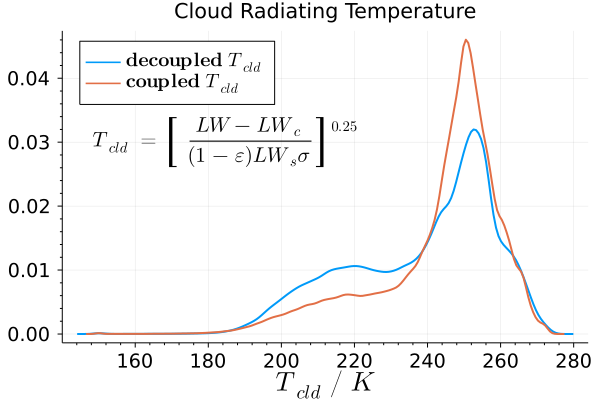
\includegraphics[width=.3\linewidth]{cloud_radiating_T.png}}\hfill
	\subfloat[c]{\includegraphics[width=.3\linewidth]{Fnet_vs_IWP_both.png}}
	\caption{[a] PDF for CRE ($F_{lw}^\downarrow$ cloudy - clear sky) shows a more frequent occurrence for cases when the clouds are coupled. [b] CRT estimated from clear-sky LW ($LW_c$), fractional sky cover ($LW_c$), indicating that warmer clouds are more frequent for coupled cases. [c] LW net radiation as a function of observed ice water path (IWP), where coupled $F_{lw}^{net}$ slightly decreasing when IWP approaches zero, contrasting to LWP where $F_{lw}^{net}$ drops strongly.}
\end{minipage}

CRE is calculated based on cloudy observations and corresponding clear-sky simulations following [\ref{bib:bruts1975}] and [\ref{bib:long2008}] for longwave downwelling radiation. Clear sky calculation is a state-of-the-art value added product from ARM~[\ref{bib:riihimaki2019}].
   
%\parbox[l]{0.8\linewidth}{   \vspace{-.5em}
%	{Some text here....}    
%}
}

%%%%%%%%%%%%%%%%%%%%%%%%%%%%%%%%%%%%%%%%%%%%%%%%%%%%%%%%%%%%%%%%%%%%%%%%%%%%%%
\headerbox{4.- Conclusions}{name=conclutions,column=1,span=2,below=results}{
  %%%%%%%%%%%%%%%%%%%%%%%%%%%%%%%%%%%%%%%%%%%%%%%%%%%%%%%%%%%%%%%%%%%%%%%%%%%%%%
{Ground-based radiation observations at the ARM site at the North Slope of Alaska (NSA) have been analyzed for the period of winters 2012 to 2020. The data has been classified into sea ice - cloud coupled/ decoupled cases. The results are consistent with previous findings regarding the effect of low sea ice concentration (e.g., due to the presence of leads or polynyas) on cloud micro- and macro-physical properties. Cloud properties like liquid and ice water path (LWP and IWP), cloud base height, and cloud geometrical thickness are also variables strongly influencing the surface radiation budget. Our results depict that a warming cloud effect on the surface is clearly enhanced by atmospheric thermodynamic and dynamic conditions which are coupled with the sea ice situation downwind.

So far only simulation of clear-sky for longwave downwelling radiation have been considered, in the future we will include complete clear-sky simulations following~[\ref{bib:ebell2020}] for the central Arctic site Ny~Alesund, thus a better picture on CRE will be achieved.
}

% \sc (this make cool big font)!

}

%%%%%%%%%%%%%%%%%%%%%%%%%%%%%%%%%%%%%%%%%%%%%%%%%%%%%%%%%%%%%%%%%%%%%%%%%%%%%%
\headerbox{5.- References }{name=references,column=1, span=2, below=conclutions}{
%%%%%%%%%%%%%%%%%%%%%%%%%%%%%%%%%%%%%%%%%%%%%%%%%%%%%%%%%%%%%%%%%%%%%%%%%%%%%%
%\colouredcircle \hspace{2em}
\hspace{-2.4em}
\begin{minipage}{0.99\linewidth}
{\scriptsize
	\begin{enumerate}
		\item \label{bib:shupe2015}Shupe, M. D. et al. "Deriving Arctic Cloud Microphysics at Barrow, Alaska: Algorithms, Results, and Radiative Closure". J. Appl. Met. and Clim. 54, 1675–1689 (2015).
		\item \label{bib:ebell2020}Ebell, K., et al. "Radiative Effect of Clouds at Ny-Ålesund, Svalbard, as Inferred from Ground-Based Remote Sensing Observations". J. Appl. Met. and Clim. 59, 3–22 (2020).
		\item \label{bib:thakur2022}Thakur, G., Schymanski, S. J., Mallick, K., Trebs, I. & Sulis, M. Downwelling longwave radiation and sensible heat flux observations are critical for surface temperature and emissivity estimation from flux tower data. Sci Rep 12, 8592 (2022).
		\item \label{bib:bruts1975}Brutsaert, W. "On a derivable formula for longwave radiation from clear skies". Water Res. Resch. 11(3): 742-744 (1975)
		\item \label{bib:long2008}Long, CN. and Turner, DD. "A method for continuous estimation of clear sky downwelling longwave flux developed using ARM surface measurements". J. Geo. Res. Atmos. 113(D18): D18206. (2008)
		\item \label{bib:riihimaki2019}Riihimaki, L. D., Gaustad, et al. "Radiative Flux Analysis (RADFLUXANAL) Value-Added Product: Retrieval of Clear-Sky Broadband Radiative Fluxes and Other Derived Values". DOE/SC-ARM-TR-228, 1569477 (2019) doi:10.2172/1569477.
		\item \label{bib:dolinar2016}Dolinar, E. K., et al. "A clear-sky radiation closure study using a one-dimensional radiative transfer model and collocated satellite-surface-reanalysis data sets". J. Geophys. Res. Atmos. 121, 13,698-13,714 (2016).
		
	\end{enumerate}
}	
\vspace{-0.6em}
\end{minipage}
	%\end{tabular}
	%\vspace{0.5em}
}
%%%%%%%%%%%%%%%%%%%%%%%%%%%%%%%%%%%%%%%%%%%%%%%%%%%%%%%%%%%%%%%%%%%%%%%%%%%%%%
\headerbox{6.- Acknowledges}{name=acknown,column=0, span=3, above=bottom}{
	%%%%%%%%%%%%%%%%%%%%%%%%%%%%%%%%%%%%%%%%%%%%%%%%%%%%%%%%%%%%%%%%%%%%%%%%%%%%%%
	{\small This work was supported by the DFG funded Transregio-project TR-172 "Arctic Amplification $(AC)^3$". The authors thanks the DOE ARM program for providing all data from the NSA site. Sea ice data is possible thanks to University of Bremen data repository and Dr. Gunnar Spreen for his collaboration. Cloud classification was performed by the open-source \emph{Cloudnetpy} algorithm by ACTRIS and FMI. }
}

\end{poster}

\end{document}

%%%%%%%%%%%%%%%%%%%%%%%%%%%%%%%%%%%%%%%%%%%%%%%%%%%%%%%%%%%%%%%%%%%%%%%%%%%%%%%
